\documentclass[12pt]{article}
\usepackage[margin=1in]{geometry}

\usepackage{wrapfig}
\usepackage{graphicx}
\graphicspath{ {figures/} }

\usepackage{enumerate}
\usepackage{enumitem}
\setlist{nolistsep}

\title{Analyzing the Clinical Microbiome \\ Biological Engineering Thesis Proposal}

\author{Claire Duvallet}
\date{October 11, 2016}

\begin{document}


\maketitle
\newpage
\tableofcontents

\begin{abstract}
Analyzing the microbiome is hard. Getting clinical insights from analyses is even harder. I'm gonna do some analyses to give us insight into an under-studied clinical microbial system, do some meta-analyses to get direly-needed biological consensus on gut microbiome and disease, and propose a new tool for analyzing 16S datasets.
\end{abstract}
\newpage

\section{Overall objectives and specific aims}
\subsection{Overall objectives}

In spite of the recent increase in research about the human microbiome, there is not a clear consensus on the relationship between human microbial communities and disease. Current 16S microbiome analyses typically study one patient cohort in one disease state, searching for individual disease-associated microbes. However, different published studies for the same disease often contain contradictory or inconsistent results. Existing meta-analyses rarely expand to more than one or two diseases, and thus do not distinguish between microbes which are associated with specific diseases from those which are associated with disease in general. Finally, there are no established tools to extract general biological insights from groups of disease-associated microbes.

This thesis will increase our understanding of the clinical microbiome by moving analyses from focusing on single microbes in individual diseases toward consolidation of groups of related microbes across many different kinds of diseases. In this thesis, I will first apply standard methods to characterize the under-studied microbiota of the aerodigestive tract of one patient cohort. Then, I will perform a comprehensive meta-analysis of gut microbiome studies across many disease states with multiple patient cohorts. Finally, I will develop a tool to enable generalizable interpretation of results from existing and future microbiome studies. This work will improve our understanding of the clinical relevance of the human microbiome and will also provide new approaches and tools for analyzing future studies.

\subsection{Specific Aims}
\begin{description}
	\item[Aim 1] Apply standard methods to identify microbial community characteristics associated with gastro-esophogeal reflux disease and aspiration.
		\begin{enumerate}
			\item Determine how lung, gastric, and throat microbial communities are related.
			\item Identify clinical modulators of lung, gastric, and throat microbial communities.
		\end{enumerate}
	\item[Aim 2] Perform a meta-analysis of case-control gut microbiome studies to identify consistent microbial signatures within and across multiple diseases.
	\begin{enumerate}
		\item Compile and process publicly available case-control gut microbiome studies using a standardized method.
		\item Identify microbes that are consistently associated with specific diseases and with disease in general.
		\item Compare results betweens studies to identify similarities in microbial characteristics of physiologically-related diseases.
	\end{enumerate}
	\item[Aim 3] Enable generalizable interpretations of microbiome analyses by assigning bacteria to groups with similar functions and known associations with disease.
	\begin{enumerate}
	\item Combine existing databases with targeted literature searches to define \textit{microbe sets} based on known biological relationships.
	\item Use machine-learning techniques to extract disease-associated \textit{microbe sets} from datasets collected in Aim 2.
	\item Develop these \textit{microbe sets} into a collaborative tool for use in interpreting new microbiome studies.
	\end{enumerate}
\end{description}
\newpage

\section{Background and significance}
\textit{Three to five pages}

The microbiome is a hot hot hot field and we know some stuff but we don't know a lot of stuff too.

My aims cover multiple body systems: aerodigestive and gut. My aims also span from one study to many, so need to talk about those approaches.

\subsection{Biological background and significance}

\subsubsection{Aerodigestive tract: physiology and disease}
Clinically, gastric and lung disorders are known to be associated but the nature of the relationship is not fully understood. For example, gastro-esophageal reflux disease (GERD) is associated with many respiratory disorders like asthma and chronic pulmonary disease (REF) and aspirators are known to be at higher risk for respiratory infections. However, the exact mechanisms of these associations remains unclear. Researchers have hypothesized that the lungs and stomach may be physically connected, with gastric contents seeding the lungs and leading to disease, and that their microbiota may be involved in causing or exacerbating disease. However, the microbial communities in human lungs and stomachs are among the least studied, except in a few specific disease (CF REF, H. pylori REF). In fact, until recently medical literature stated that the lungs were sterile and free of bacteria (REF). Neither gastric nor lung sites were included in the Human Microbiome Project, leading to a dearth of studies and data on these important body sites.

First, we will investigate how much of the throat, gastric, and lung microbial communities are shared across sites. From an engineering perspective, the stomach, throat, and lungs can be thought of as different compartments connected by the esophagus and windpipe. (FIGURE) The mass transport between these compartments is regulated by complex physiological mechanisms. Swallowing guides material from the mouth to the stomach, but may dysfunction and allow material to enter the lungs. The esophageal sphincter usually prevents material from leaving the stomach, but in some diseases is dysfunctional. Finally, complex homeostatic mechanisms clear the lungs of foreign bodies and create a very selective environment for microbes in the lungs (REFS REFS REFS). Thus, while the throat, stomach, and lung "compartments" are physically connected, the amount of material, including bacteria, flowing between them is not readily apparent. Before investigating how clinical factors can modulate the microbiota in the stomach, lungs, and throat, we must first determine how much exchange of microbial communities can and does happen between these sites.


\subsubsection{Microbiome of the aerodigestive tract}
It's all super complicated, yo. And also super connected wat who knew.


Only one previous study has examined the relationship between sites of the upper aerodigestive tract (REF). Bassis et al. found that oral microbial communities were more similar to both stomach and lung communities than nasal communities. However, these authors did not examine the inter-relationships between all sites - their driving hypothesis was that the mouth is the source of the downstream communities. In this work, we will take a broader view: which of the upper aerodigestive body sites exchange microbes, are these the same microbes across multiple patients, and are there phylogenetic patterns for these shared microbes? 


\subsubsection{Lower gastrointestinal tract: physiology and disease}
Stuff about all the disease I'll be looking at - vaguely.

\subsubsection{Microbiome of the lower gastrointestinal tract}
We know way more, and also not that many hard and fast conclusions.

\subsection{Analytical background and significance}
Start with summary of how we get from sample to data.
16S is in all bacteria, we amplify a conserved part of that 16S and sequence it using NGS. This gives us lots of data, which we quality filter and assign taxonomy.
Make sure to define what an OTU is here!!

Then talk about what we do with the data.

\subsubsection{Current analytical approaches for 16S analyses}
Including how community related-ness is measured.

Common methods: Alpha diversity, JSD, t-tests, etc
Data analysis: lots of multiple corrections to do

Data processing: different methods (OTU calling, Latin name mapping) lead to drastically different results

What studies exist, sample size limitations, different technologies, batch effects.

\subsubsection{Existing meta-analyses}
Haven't found much and haven't been great.

\subsubsection{Databases and tools for annotations}
GSEA is commonly used in RNAseq data! Gene databases exist and have been curated into gene sets.
No curated microbe sets. Some existing similar tools: SourceTracker, ImG, ...?

\section{Research design and methods}
\textit{Six to eight pages}

\subsection{Aim 1: Aerodigestive microbiota associated with GERD and aspiration}

\begin{wraptable}{r}{5.5cm}
\begin{tabular}{|l|c|}
	\hline
	\textbf{Sites} & \textbf{N} \\
	\hline
	gastric, throat, \& BAL & 87 \\
	gastric \& throat & 45 \\
	gastric \& BAL & 34 \\
	BAL \& throat & 9 \\
	\hline 
\end{tabular}
\caption{Aerodigestive site samples}\label{tab:rosen_samples}
\end{wraptable}

As discussed previously, patients with aerodigestive disorders like aspiration and GERD are at a higher risk for respiratory infections. We hypothesize that microbial communities in the aerodigestive tract share and exchange certain members which then contribute to infections, and that clinical factors like reflux or aspiration disease change the amount of bacterial exchange between aerodigestive sites.

Our patient cohort consists of 261 patients recruited by Rachel Rosen (M.D., GI/Nutrition) at Boston Children's Hospital for multiple studies over the course of the past 6 years. Multiple samples were taken from patients: throat swabs, gastric fluid, and broncho-alveolar lavages (BAL) (Table \ref{tab:rosen_samples}). 125 patients were monitored for full-column GERD and 112 patients were tested for aspiration. Overall, this cohort represents the largest existing human aerodigestive microbiome dataset.


\subsubsection{Exchange of microbes between lung, gastric, and throat communities} \label{sec:exchange}
To understand the microbial exchange between sites in the aerodigestive tract, we will first define a metric to quantify how "shared" microbes are between two sites. There are multiple ways to define this metric: as the percentage of patients who have the microbe present in both sites, as the correlation between the abundance of the microbe in one site with its abundance in the other site, or some combination of these two approaches. Because many microbes in the stomach and lungs are seeded by the oral community, simple co-occurence of bacteria is not sufficient to establish meaningful microbial exchange (REF). Using the correlation of abundances in two sites is also not adequate, since many people may not have the OTU present in either or both sites due to the inherent variability of microbial communities between people.

Thus, we will use both co-occurence and correlation to quantify microbial exchange across sites, which we call $p_s$. We will first identify which microbes are shared using the abundance correlation, and then quantify each microbe's degree of sharedness by its co-occurence rate in patients. For each microbe, we will calculate the non-parametric Spearman rank correlation of the log10(relative abundances) in the two sites, using only abundances from patients with the microbe present in both sites. If this correlation is greater than 0.5, the microbe is considered to be shared. Our metric $p_s$ is then defined as the percentage of patients who have the microbe present in both sites (Fig. \ref{fig:sharedness_defn}).

\begin{wrapfigure}{R}{0.5\textwidth}
	\centering
    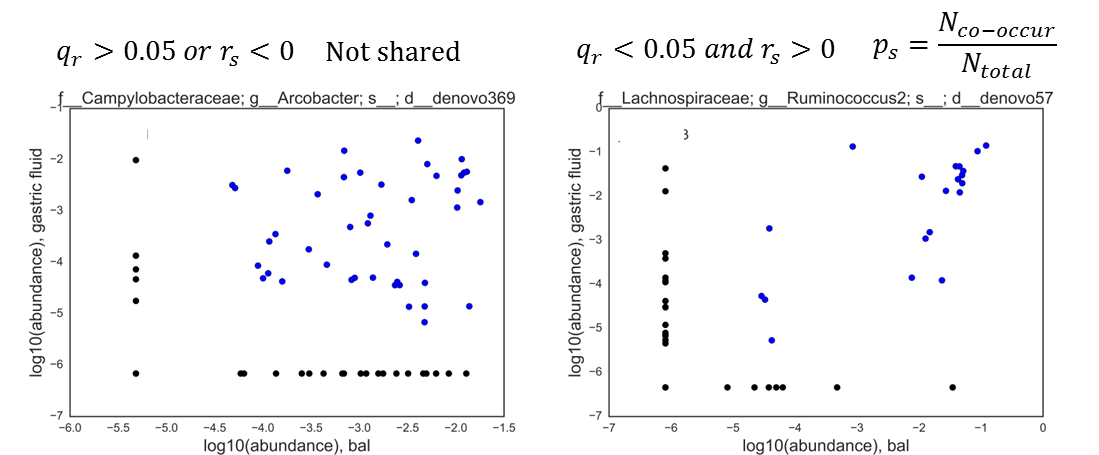
\includegraphics[scale=0.5]{sharedness_definition}
    \caption{Determining $p_s$}\label{fig:sharedness_defn}
\end{wrapfigure}


\subsubsection{Clinical modulators of lung, gastric, and throat microbial communities}
Once we quantify microbial exchange within the aerodigestive tract, we can begin to ask which clinical factors modulate how much exchange occurs between sites. We will calculate $p_s$ for all a-priori defined exchanged microbes (Section \ref{sec:exchange}), stratified by the clinical factor. Furthermore, we will investigate whether the total abundance of exchanged microbes in the different sites and beta diversity community similarities differ between our case and control patient groups.

Our first hypothesis is that aspirators will have a stronger connection between their throat and lungs. Additionally, because many of these patients have GERD, we also expect a slight increase in the connection between the stomach and lungs. Our dataset has 48 patients with abnormal MBS test results (Aspirators) and 63 patients with normal results.

Our next hypothesis is that patients with more severe GERD will have more sharing between the stomach and lung communities. Because are interested in GERD that may modulate the stomach-lung connection, we define "severe GERD" as reflux in which more than 50\% of events are full-column reflux events. With this definition, we have 99 patients with severe GERD and 26 patients without. In addition to the binary severe/not severe comparison, we may regress each of the continuous measures of GERD severity onto the abundance of microbes in each patient's lung and stomach communities. We will also investigate how PPIs modulate the connection between aerodigestive sites, since PPIs are often prescribed for respiratory disease but have unclear clinical impact. The dataset has 114 patients on PPIs and 85 patients not on PPIs.

\subsubsection{Additional considerations}
One factor to consider when drawing conclusions from the $p_s$ metric is that because of the low bacterial biomass in the gastric and lung sites, it is possible that some microbes which are "exchanged" across these sites are simply both being seeded by the environment. However, if these microbes are phylogenetically related or they are known members of the gastric or lung communities, this would indicate that the OTUs are being selected for by the environment and are relevant community members.

This work does not address the direction of microbial exchange between aerodigestive sites, nor does it directly link increased microbial exchange with adverse outcomes like respiratory infections. Follow up studies focus on patients who develop respiratory infections, or patients who frequently have GERD- or aspiration-associated respiratory infections. 

Finally, an important caveat to note when discussing the human lung and gastric microbiomes in general is that our basic understanding of these communities in healthy humans is still quite rudimentary. For example, the extent to which lung microbial communities are composed of surviving and replicating microbes versus transient members is unknown. However, because we do see similarities in microbiota across patients, we can conclude that at least some selection is happening in these sites, and even if these communities are not thriving they may still be physiologically relevant.

\subsection{Aim 2: Meta-analysis of gut microbiome studies}
By combining results from existing gut microbiome case-control studies, we can move the field toward a consolidated understanding of consistent microbial markers of gut-related diseases. We hypothesize that certain bacteria will often be associated with disease, and that some of these bacteria will be associated with many different types of diseases while others will be unique to one or two conditions. Additionally, we hypothesize that microbial signatures  of health and disease will be more similar in similar diseases (i.e. diabetes and obesity).

\subsubsection{Compile and process gut microbiome datasets}
To perform a comprehensive meta-analysis, we need to collect a comprehensive selection of 16S gut microbiome case-control studies. We will identify these studies through a targeted literature search.  See TABLE for exclusion and inclusion criteria for studies to be considered.

We will process these datasets using a standardized in-house pipeline developed by Thomas Gurry and to which I have contributed. We will start with the rawest available data - in most cases, these will be fastq files but for some studies we will begin from quality-filtered fasta files. Sequences will be quality and length trimmed, clustered at 100\% similarity, and assigned Latin taxonomic names using the RDP classifier. Samples with fewer than 100 reads will be removed from consideration. OTUs with fewer than 10 reads or which are present in less than 1\% of samples will be removed. More stringent quality filtering may be considered in order to reduce noise in the dataset.

Because studies which sequence different 16S regions will have different sequences corresponding to the same bacteria, we can not used sequence-based open-reference approaches to compare OTUs across studies. After assigning Latin names based on OTUs within each study, we will collapse OTUs to the genus level and compare these across studies.

\subsubsection{Identify microbes consistently associated with diseases}\label{sec:indep_studies}
Once we have processed all datasets in a standardized way, our first goal is to identify consistent markers of health and disease. We will analyze each dataset with methods commonly used in the literature: univariate non-parameteric statistical tests on relative abundances, alpha and beta diversity in different types of patients, and ratios of Firmicutes to Bacteroides in healthy vs. disease patients. It is generally thought that low alpha diversity is a marker of dysbiosis (REF), and that while most people have a Firmicutes/Bacteroides ratio of (XXX), in certain diseases this ratio may be different (REF). (MAYBE BACKGROUND?) By analyzing each study in the same way from raw data, we can reduce the study-wise batch effects and increase our ability to identify general trends in the gut microbiome in health and disease.  

\subsubsection{Compare results between studies for related diseases}
Our next hypothesis is that similar diseases will have similar signatures of dysbiosis. For example, we expect that metabolic diseases like obesity and diabetes will have more similar microbiota disruptions than they will to diarrheal diseases like Clostridium difficile infection or enteric diarrhea. 

We will summarize each dataset with one vector indicating its "microbial signature". This signature will be based on number and identities of microbes significantly associated with the disease and the direction of change of these microbes. Depending on the results from Section \ref{sec:indep_studies}, we may also include factors like differences in alpha diversity or Bacteroides/Firmicutes ratios. Then, we will investigate which diseases cluster together in this "signature space". (SEE FIGURE WITH PCA FLOWCHART) 

If a disease has a strong impact on or association with the gut microbiome, then we would expect its signatures from multiple studies to cluster very tightly together. If this is the case, we can extract the bacterial features which contribute the most to this tight clustering - these will then be most likely to be associated with that specific disease, and would be good candidates for further mechanistic explorations. On the other hand, if datasets of the same disease or similar conditions do not have similar microbial signatures, this may indicate that the microbiome is not inherently implicated or affected by the disease. In this case, any signal that we see in the gut microbiome is likely driven by other non-disease effects, which are not necessarily the same across studies. Finally, if we find different diseases with similar underlying causes (i.e. inflammation) clustering relatively near each other, then perhaps this would indicate that the microbiome is affected or involved with the underlying cause rather than the specific diseases. Such insights could help us design better experiments to follow up on mechanism or causal relationships.

\subsubsection{Additional considerations}
Although some mechanistic studies have reported consisted bacterial associations with diseases like colorectal cancer and IBD (REFS), it is possible that we struggle to find bacteria consistently associated with diseases because of technical batch effects. In this case, we could consider using a phylogenetics-based approach: rather than looking for specific genera associated with diseases, we can identify associations with open-referenced OTUs and then compare their phylogenetic relationships across all studies. Another approach could be to use tools like PiCRUST to assign functionality to our observed taxonomies, and approach these analysis from a functional point of view.


Another important consideration in this work may be if study-associated effects are larger than biological effects. For example, when we compare 'microbial signatures' across datasets, it's possible that the largest signal driving dataset clustering is sequencer or 16S region sequenced, rather than disease state. There are many approaches we could take to correct for such batch effects:
\begin{enumerate}
	\item Subtracting the principal components corresponding to the technical artifact
	\item Build a model that accounts for these technical artifacts by including them as factors in the model.
	\item Transform the data in ways shown to remove batch effects, cumulative sum normalization (HAS IT BEEN SHOWN TO REMOVE BATCH EFFECTS??).
	\item Non-parametric correction, like sample- or OTU-wise quantile normalization, using controls in each study as the reference distribution.
\end{enumerate}

\subsection{Aim 3: Assigning bacteria to groups with similar functions and disease associations}

\subsubsection{Define microbe sets based on known biological relationships}
Using an undergrad and lots of lit searching. And ImG and Ilana.

\subsubsection{Extract disease-associated microbe sets from datasets in Aim 2}
And \#machinelearning stuff bam wow wow.

\subsubsection{Develop collaborative tool for interpreting microbiome studies}
See if results jive with what we found from individual genus-based analyses, if we uncover new "signatures of general types of diseases", etc.

\subsubsection{Additional considerations}

\section{Preliminary studies}
\textit{Three to four pages}

\subsection{Aim 1}
\subsubsection{Microbiome community sharedness}
Look what I can do ma.

\subsubsection{Modulators of sharedness}
And here!

\subsection{Aim 2}
\subsubsection{Collect datasets}
Check out what I got!

\subsubsection{Find consistent microbes}
PCA, alpha diversity, comparing microbial signatures, consistency of significant OTUs.

\section{Conclusion}

\section{Gud werds}
We hypothesize that there is a clinically-relevant exchange of bacteria within the aerodigestive tract that may be altered in certain disease states. 

\end{document}